%examples
\section{样例}
\subsection{阴影}\label{yl:yy}
\begin{itemize}
\item 传统操作
\begin{description}
\item[关键点] 三个图层
\begin{description}
\item[背景图层] 一般用白色或透明,用来反衬实景图层
\item[阴影图层] 在实景图层的基础上,用四次高斯模糊滤镜,并往右下方移动4个像素
\item[实景图层] 具体的实景
\end{description}
\item[主要命令] 路径[B],油漆桶填充[shift+B],混合填充[L],移动[M],高斯模糊滤镜
\item[具体操作]
图层结构如下图\ref{yl:yy:layers}:
\begin{figure}[!htbp]
	\centering
	\caption{图层结构}
    	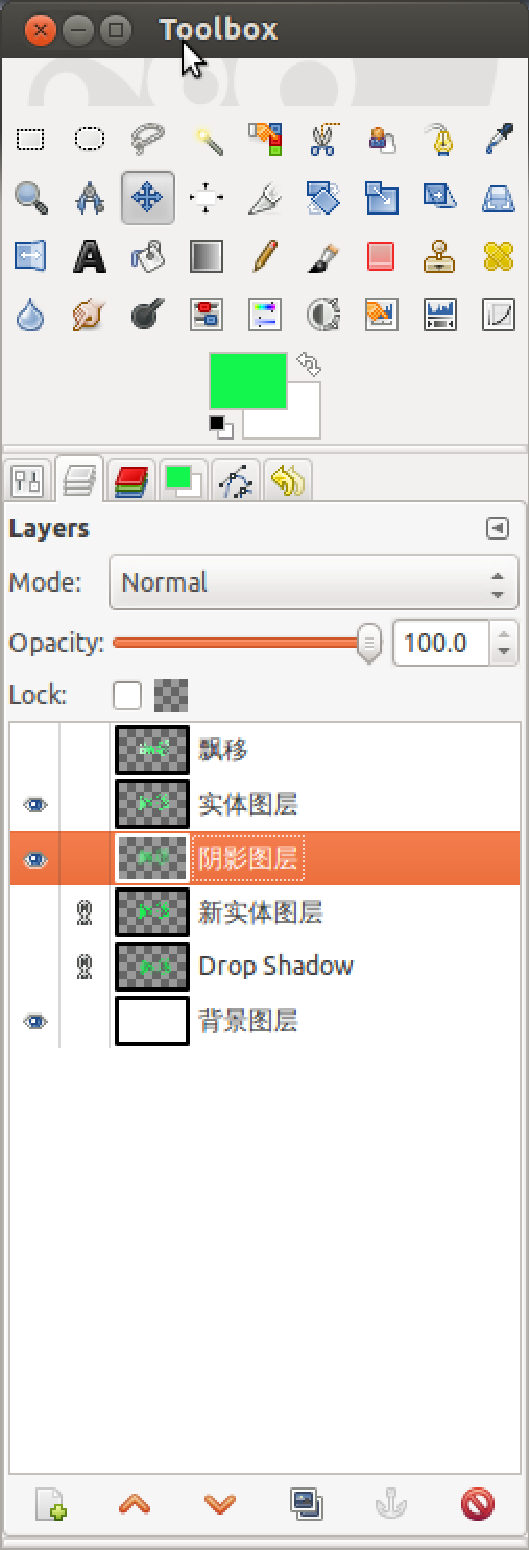
\includegraphics[scale=0.4]{figs/yy-layers.pdf}
    	\label{yl:yy:layers}
\end{figure}
\end{description}
\item 新操作 \\
通过gimp的最新版本中包含的阴影滤镜(drop shadow),可以直接生成阴影.参数设置如下图\ref{yl:yy:set}
\begin{figure}[!htbp]
	\centering
	\caption{阴影滤镜参数设置}
    	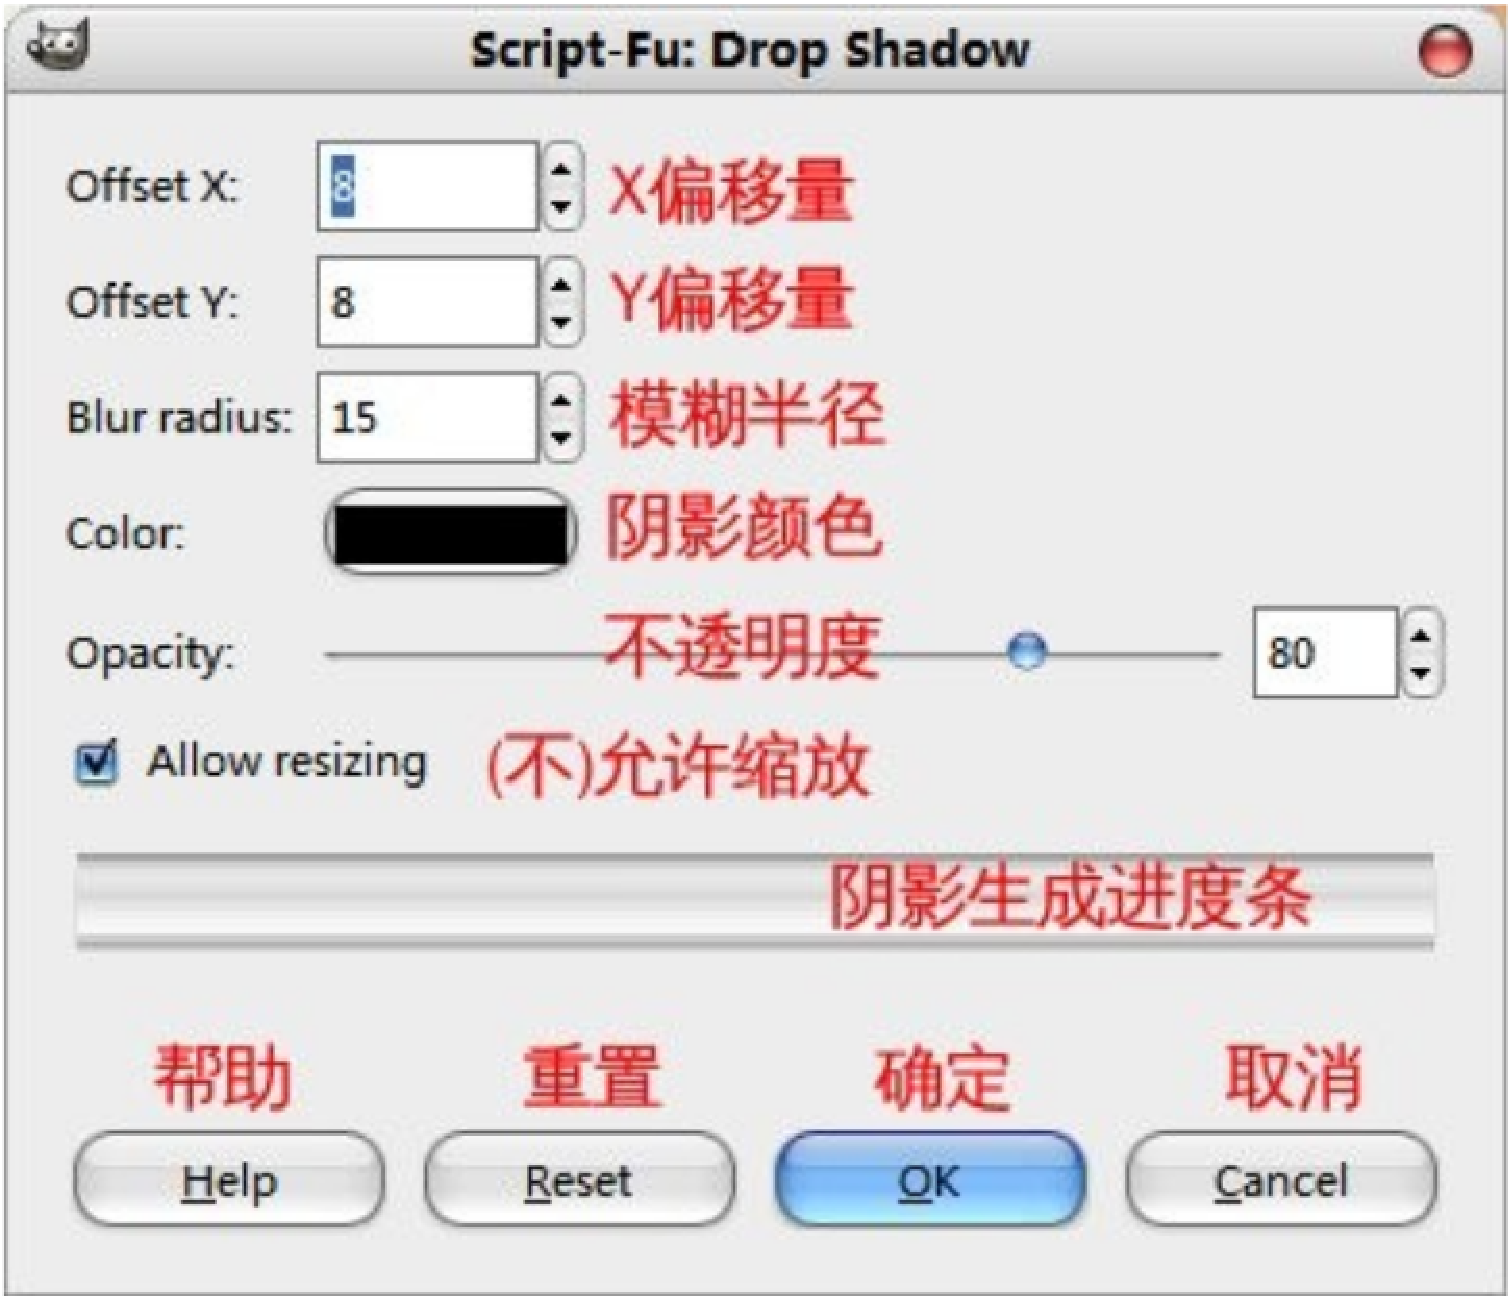
\includegraphics[scale=0.4]{figs/yy-set.pdf}
    	\label{yl:yy:set}
\end{figure}
\end{itemize}

\clearpage

\subsection{金属拉丝}\label{yl:zsls}
\begin{description}
\item[关键点] 
\begin{description}
\item[RGB噪音] 详见RGB噪音\ref{filters:noise:rgb}
\item[高斯模糊] 详见高斯模糊\ref{filters:blur:gaussian}
\end{description}
\item[主要命令] 油漆桶填充[shift+B],高斯模糊,RGB噪音
\item[具体操作]
图层结构如下图\ref{yl:zsls:layers}:
\begin{figure}[!htbp]
	\centering
	\caption{图层结构}
    	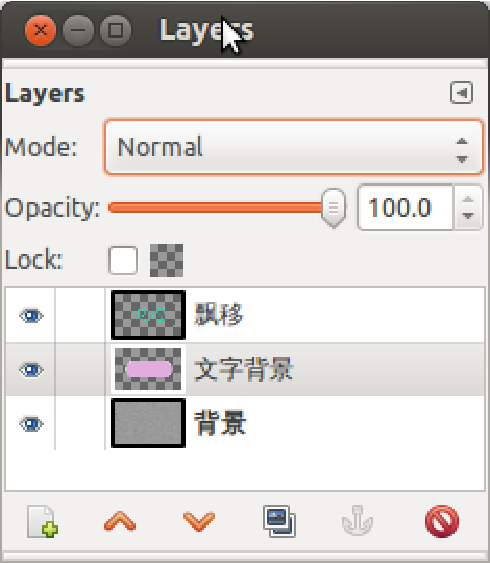
\includegraphics[scale=0.4]{figs/zsls-layers.pdf}
    	\label{yl:zsls:layers}
\end{figure}
效果如下图\ref{yl:zsls:results}:
\begin{figure}[!htbp]
	\centering
	\caption{金属拉丝效果}
    	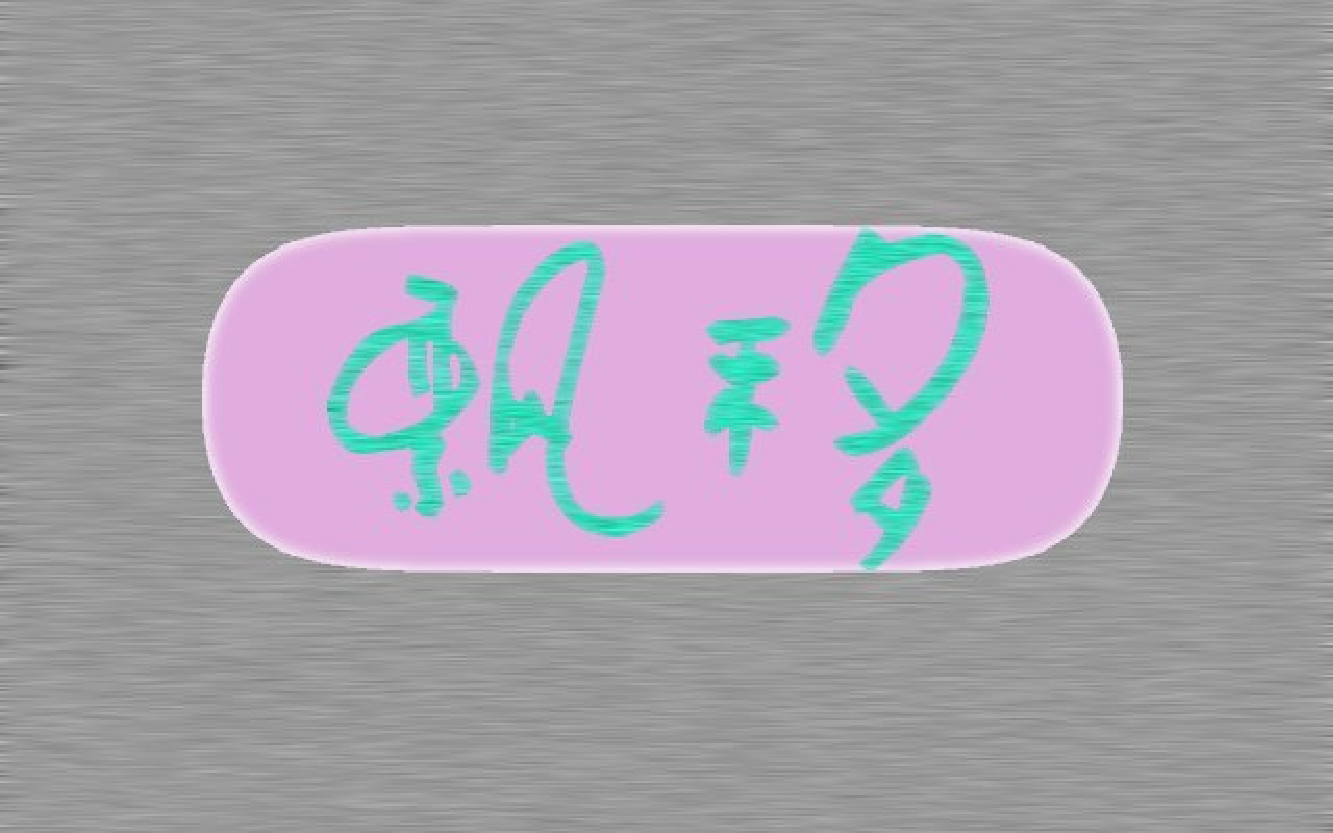
\includegraphics[scale=0.4]{figs/zsls-results.pdf}
    	\label{yl:zsls:results}
\end{figure}
\end{description}





\clearpage